
\section{Lecture 1: Units, dimensions and scaling arguments}
\begin{figure}[H]
  \centering
  \begin{tabular}{ | p{5cm} | p{3cm} | p{2.5cm} | p{2cm} | }
    \hline
    \rowcolor{black}
    \multicolumn{4}{|c|}{\color{white}SI Base Units} \\
    \hline
    \hline
    \rowcolor{darkgray}
    \multicolumn{2}{|l|}{\color{white}Base quantity} & \multicolumn{2}{l|}{\color{white}Base Units} \\
    \hline
    \rowcolor{lightgray}
    Name & Typical symbols & Name & Symbol \\  
    \hline
    \rowcolor{yellow}
    time & $t$ & second & $\SI{}{\second}$ \\  
    \hline
    \rowcolor{orange}
    length & $l, x, r,$ etc. & meters & $\SI{}{\meter}$ \\
    \hline
    \rowcolor{red}
    mass & m & kilogram & $\SI{}{\kilogram}$ \\
    \hline
    \rowcolor{green}
    electric current & $I, i$ & ampere & $\SI{}{\ampere}$ \\
    \hline
    \rowcolor{cyan}
    thermodynamic temperature & $T$ & kelvin & $\SI{}{\kelvin}$ \\
    \hline
    \rowcolor{magenta}
    amount of substance & $n$ & mole & $\SI{}{\mol}$ \\
    \hline
    \rowcolor{Orchid}
    luminous intensity & $I_v$ & candela & $\SI{}{\candela}$ \\
    \hline
  \end{tabular}
  \caption{Credits go to NIST SP 330.2019, Table 2.} %https://www.nist.gov/pml/owm/metric-si/si-units
  \label{fig:SI-UNITS}
\end{figure}

\begin{figure}[H]
  \centering
\begin{tabular}{l c S[table-format=10.9] S[retain-zero-exponent=true]}
  \toprule
  \multicolumn{4}{c}{SI Prefixes} \\
  \addlinespace %\midrule
  Prefix & Symbol & {Multiplication Factor} & {\dots\ in Scientific Notation} \\
  \midrule
  giga  & \si{\giga} & 1000000000 & e9 \\
  mega  & \si{\mega} & 1000000    & e6 \\ 
  kilo  & \si{\kilo} & 1000       & e3 \\
  deca  & \si{\deca} & 10         & e1 \\ % "\deka" works too
  \rowcolor{gray!20}  -- & -- & 1 & e0 \\
  deci  & \si{\deci} & 0.1        & e-1 \\
  centi & \si{\centi}& 0.01       & e-2 \\
  milli & \si{\milli}& 0.001      & e-3 \\
  micro & \si{\micro}& 0.000001   & e-6 \\
  nano  & \si{\nano} & 0.000000001& e-9 \\
  \bottomrule
  \end{tabular}
  \caption{}
  \label{fig:SI-PREFIX}
\end{figure}

In dimensional analysis we use squared brakets to denote \textit{units} 
but a \textit{dimension} we use parenthesis, e.g.,  $[t]$ or $(s)$. They are 
shown in Table~\ref{fig:SI-UNITS} and can be combined with the SI Prefixes in 
shown in Table~\ref{fig:SI-PREFIX}.

Many other units can be described as combinations of the three base units shown above, for example:

\begin{equation}
 \text{[speed]} = \frac{\text{[l]}}{\text{[t]}}
\end{equation}

All units of speed are in length per time - meters per second, kilometers per hour, inches per year, etc. Therefore, we say that the \emph{dimension} of speed is the dimension of length per time, as shown above in a more mathematical notation.

Other examples are:

\begin{equation}
 \text{[volume]} =\text{[l]}^3
\end{equation}
\begin{equation}
 \text{[density]} = \frac{\text{[m]}}{\text{[l]}^3}
\end{equation}
\begin{equation}
 \text{[acceleration]} = \frac{\text{[l]}}{\text{[t]}^2}
\end{equation}

The last one may seem strange if you have not studied physics before - an example of a unit of acceleration is meters per second squared, or meters per second per second ($m/s^2$ or $(m/s)/s$). It's quite simple though, once you get past the wording of it.\\
When measuring a change in something, we always add another "per second" (or another unit of time), so when the unit we are measuring the change in is already meters per second, we get meters per second per second.\\
For example, a car might start out at 0 m/s (standing still), and be moving at 5 m/s one second later. In that case, the car's average acceleration is 5 meters per second per second.

\subsection{Uncertainty}
Prof. Lewin stresses very strongly: ``Any measurement you make without knowledge of its uncertainty is \emph{meaningless}''. He repeats this a few times throughout the lecture.
First, keep in mind that some numbers are exact. If we multiply a length by 2 -- a constant, not a measurement -- then the length and the uncertainty are both multiplied by 2 exactly. No further work is necessary.\\

\subsubsection{Uncertainty in addition and subtraction}

For addition and subtractions, it couldn't be much easier: the uncertainty of the sum or difference is simply the sum of the two uncertainties:

\begin{equation}
 (A \pm a) + (B \pm b) = (A + B) \pm (a +b)
\end{equation}
\begin{equation}
 (A \pm a) - (B \pm b) = (A - B) \pm (a +b)
\end{equation}

You can find this result by calculating with the extremes. For example, for adding $1.5 \pm 0.003 \text{ m} + 3 \pm 0.005 \text{ m}$:

\begin{equation}
\text{min} = 1.497 \text{ m} + 2.995 \text{ m} = 4.492 \text{ m}
\end{equation}
\begin{equation}
\text{max} = 1.503 \text{ m} + 3.005 \text{ m} = 4.508 \text{ m}
\end{equation}

Both results are $0.008$ m away from $3 + 1.5 = 4.5$, and so the uncertainty is $\pm 0.008$ m, the sum of the two uncertainties.  
If we use the same method where we subtract, we will find the same result: the uncertainties \emph{add}, and the results will differ from the simple difference by $+0.008$ and $-0.008$, respectively.

\subsubsection{Uncertainty in multiplication and division}
One way to get a \emph{rough} uncertainty value when dividing is to choose the largest and smallest values, respectively, for the numerator and denominator, and then subtract the nominal value from that.\\
As an example, let's say we want to calculate the approximate gravitational acceleration of the Earth based on measurements of the time for an object to fall from a certain height. The equation used is

\begin{equation}
 g = \frac{2 h}{t^2}
\end{equation}

The 2 here is an exact value, so we don't need to worry about it.\\
If the height is $\SI{3.000(3)}{m}$ and the time taken is $\SI{0.781(2)}{s}$, we then find:


\begin{equation}
g = \frac{2\cdot\SI{3.000}{m}}{(\SI{0.781}{s})^2} \approx \SI{9.8367}{m/s^2} \approx \SI{9.84}{m/s^2}
\end{equation}

We can then calculate the uncertainty as mentioned above. For the numerator, we add the $+ 0.003$ m, and in the denominator, we subtract the $- 0.002$ s. Finally, we subtract the nominal value that we found above.

\begin{equation}
\text{error} = \frac{2 \cdot \SI{3.003}{m}}{(\SI{0.779}{s})^2} - g = \SI{9.8971}{m/s^2} - \SI{9.8367}{m/s^2} = 0.0604 \approx \SI{0.06}{m/s^2}
\end{equation}



\subsection{Dimensional analysis}

Let's do a dimensional analysis of how long it takes to drop and object on earth.
Most likely the time $t$ depends on the height $h$ to some unknown power $\alpha$, i.e., $t \propto h^\alpha$.
If we did not know any better we might think mass $m$ has an effect with some unknown power $\beta$.
This gives us $t \propto h^\alpha m^\beta$. We also would think that gravity $g$ has an effect with a power of $\gamma$. 
That leaves us with $t \propto h^\alpha m^\beta g^\gamma$

We can now start trying to figure this out. We know that the left-hand side has the dimension of time, [T]. This means that the product on the right-hand side must also have the dimension of time. Using the dimensional analysis notation, we must have

\begin{align*}
  &\text{[T]}^1 = \text{[L]}^\alpha \text{[M]}^\beta \left( \frac{\text{[L]}}{\text{[T]}^2} \right)^\gamma  \\
  &\rightarrow \beta=0, \alpha+\gamma=0, -2\gamma = 1 \\
  &\rightarrow \gamma = -\frac{1}{2} \rightarrow \alpha=-\gamma=\frac{1}{2} \\
\end{align*}

And, so, we find these values, and these relationships with the variable names we had chosen earlier:

\begin{align}
t &\propto h^{1/2} g^{-1/2} \\
t &\propto \sqrt{\frac{h}{g}}
\end{align}

Since the meaning of a proportionality is that some (still unknown) constant multiplies the value, we can write this as an equality with an unknown constant $C$:

\begin{equation}
 t = C \sqrt{\frac{h}{g}}
\end{equation}

So, since the time is proportional to the square root of the height, we can tell than if we drop an object first from 2 meters, and then from 8 meters, it will take twice as long to fall the second time, despite the distance being 4 times as long (because $\sqrt{4} = 2$).

\subsection{An experiment}

This is then put to the test in the lecture, by dropping apples, and timing their fall. One drop was from 3 meters, $\pm 0.003$ meters, while the second was from 1.5 meters, also with $\pm 0.003$ meters as the uncertainty.

The ratio between the two is easily calculated as 2, but what about the uncertainty? If the numerator were $3.003$ m and the denominator $1.497$ m, those would give the largest ratio possible with the uncertainty of $\pm 0.003$. The result of that division is $2.006$, so we consider the uncertainty to be $0.006$:

\begin{equation}
 \frac{h_1}{h_2} = \frac{3.000 \pm 0.003 \text {m}}{1.500 \pm 0.003 \text{ m}} = 2.000 \pm 0.006
\end{equation}

Note that because this is a ratio between two lengths, the end result has no dimension and thus no unit.

Knowing this ratio, we can now predict the ratio between the fall times. Since the ratio between the heights is 2, and the time is proportional to the square root of the height, the ratio between the fall times should be about $\sqrt{2}$. Then there's that uncertainty again. We can use the same method to find the smallest possible and the largest possible result by calculating $\sqrt{2+0.006}$ and $\sqrt{2-0.006}$ and will find an uncertainty of about $\pm 0.002$. That gives us

\begin{equation}
 \frac{t_1}{t_2} = \sqrt{\frac{h_1}{h_2}} = 1.414 \pm 0.002 \label{eq:applepred}
\end{equation}

So, the above is our \emph{prediction}, and we have a set-up with the apple fall times being measured automatically. Let's see the results!

The apple falling from 3 meters $\pm 3$ mm took $0.781 \pm 0.002$ seconds to fall. The apple falling from 1.5 meters $\pm 3$ mm took $0.551 \pm 0.002$ seconds to fall.

If we then calculate the ratio between the two times, we find

\begin{equation}
\frac{0.781 \pm 0.002}{0.551 \pm 0.002} = 1.417 \pm 0.008
\end{equation}

... which is in agreement with the prediction in \eqref{eq:applepred} when we consider the uncertainties in our measurements. \emph{Physics works}, as Prof. Lewin would say.\\
As far the uncertainty of the above result goes, I get $\pm 0.009$ when calculating the same way as before. However, as mentioned before, this method is not truly correct, and the truly correct way is out of the scope of this course, so such a small difference does not matter.\\
As long as the uncertainty is 0.001 or more, the results can agree with each other.

\section{Lecture 2: Introduction to Kinematics}

\subsection{Distance vs displacement and velocity vs speed}
Speed is a scalar, i.e., a number/cuantaty, of how fast your going in any given direction. 
The velocity is a vector containing the speed and direction.
\begin{align}
 \text{speed} &= \frac{\text{distance traveled}}{\text{time taken}}\\
 \text{velocity} &= \frac{\text{displacement}}{\text{time taken}}
\end{align}

Speed is always positive, since it does not care about the direction.
However, since velocity depends on displacement, i.e., starting point to end point,
the direction also caries the sign, which means that velocity can be negative.


\subsection{Kinematics}

We can now introduce a definition for the \emph{average velocity} of this object between two times $t_1$ and $t_2$ as the following:

\begingroup
\large
\begin{align*}
 \overbar{v}_{t_1 t_2} = &\frac{x_{t2} - x_{t1}}{t_2 - t_1} \\
 &\text{or} \\
 \overbar{v} = &\frac{\Delta x}{\Delta t}
\end{align*}
\endgroup


\subsubsection{Instantaneous velocity}

Since the definition of velocity we've seen thus far is only an average between two points in time, what is the meaning of instantaneous velocity (which is usually what we mean by ``velocity'' unless otherwise specified)?\\
Conceptually, the answer is that it is still an average, only that we move the two position measurements closer and closer together in time, until the time between them is zero.

Mathematically, velocity is the first \emph{derivative} of position.
We could write it as

\begingroup
\large
\begin{equation}
 v_t = \lim_{\Delta t \to 0} \frac{x_{t + \Delta t} - x_t}{\Delta t} = \frac{dx}{dt} = x'(t) = \dot{x}
\end{equation}
\endgroup

The last three are just three different ways of writing the same thing: the first derivative of $x$ with respect to $t$. Leibniz' notation looks like a fraction; Lagrange's notation uses the prime symbol (apostrophe) to indicate a derivative, and finally Newton's notation uses a dot above to signify the first time derivative. (In other words, the dot notation is used almost exclusively when the function is differentiated with respect to time, so the $t$ is implicit.)

As for speed, we can simply define instantaneous speed as the absolute value of the instantaneous velocity. In other words, if the velocity has a minus sign, remove it. If not, the two are equal.


\subsection{Calculating the average speed of a bullet}

Let's say we have a rifle that fires a bulet that brakes a wire that 
starts the mesurment and then another wire that stops the mesurment.
The distance between the wire was messured to be $148.5 \pm 0.5$ cm, that is, $1.485 \pm 0.005$ m.\\
The time taken was measured as $5.8 \pm 0.1$ ms, which equals, $0.0058 \pm 0.0001$ s.

The average speed is then

\begin{equation}
v_{avg} = \frac{\SI{1.485}{m}}{\SI{0.0058}{s}} = \SI{256}{m/s}
\end{equation}

The relative error in the timing can be calculated as 

\begin{equation}
\text{relative error} = \frac{\SI{0.1}{ms}}{\SI{5.8}{ms}} \cdot 100\% = 1.7\% 
\end{equation}

The timing error is much higher than the error in the distance so we can ignore the latter.

The uncertainty in the average speed can then be estimated. As the lecture question hints, we will ignore the uncertainty due to error in the distance measurement, because the timing error is much greater.

We can use the simple way introduced previously to find an approximate uncertainty:

\begin{equation}
\text{error} = \frac{1.485 \text{ m}}{0.0058 - 0.0001 \text{ s}} - \SI{256}{m/s} = \SI{4.5}{m/s}
\end{equation}

(We would add $+0.005$ m at the top, if we didn't choose to ignore the uncertainty it that measurement.)\\
Alternatively, we could have simply used the 1.7\% relative error we found above.\\
So in short, we can specify the average speed of the bullet as

\begin{equation}
v_{avg} = 256 \pm 4.5 \text{ m/s}
\end{equation}

\subsection{Acceleration}

Just as velocity is the change in position, acceleration is the change in \emph{velocity}. We can use an equation that looks extremely similar to find the \emph{average} acceleration $a$:

\begingroup
\large
\begin{equation}
 \overbar{a}_{t_1 t_2} = \frac{v_{t2} - v_{t1}}{t_2 - t_1}
\end{equation}
\endgroup

The dimension of acceleration, as mentioned previously, is length per time${}^2$, or [L] [T]${}^{-2}$, with $\text{m/s}^2$ being the most common unit, at least in this course.

Just as before, we can simplify this by using delta notation.

\begin{equation}
\overbar{a} = \frac{\Delta v}{\Delta t}
\end{equation}

Let's do an experiment where we have an ball that is throught towards the ground.
We define the direction of increasing $x$ as upwards (towards the sky). A tennis ball is thrown towards the ground at a velocity of about $\SI{-5}{m/s}$ - i.e. the speed is 5 m/s, downwards. It is in contact with the ground for about 1/100 second, after which it is moving at $\SI{+5}{m/s}$, i.e. upwards.\\
What is the average acceleration of the tennis ball?

\begin{equation}
 \overbar{a_{ball}} = \frac{\SI{5}{m/s} - (\SI{-5}{m/s})}{\SI{0.01}{s}} = \frac{\SI{10}{m/s}}{\SI{0.01}{s}} = \SI{1000}{m/s^2}
\end{equation}

Keeping the signs in mind, we end up with a positive value for the acceleration, which has a ridiculous magnitude - over 100 times the Earth's gravitational acceleration.

The professor adds another example of acceleration. There is a limit to the amount of acceleration things can tolerate before they break. He used examples of tomatoes and eggs, also thrown to the ground at 5 meters per second.\\
The impact time will probably be much greater (perhaps 1/4 second), and the change in velocity will be only 5 m/s rather than 10, as neither the egg nor the tomato would bounce back up.\\
Despite that, clearly, both would break, even though the acceleration is a more modest $20 \text{ m/s}^2$ or so.


\subsubsection{Instantaneous acceleration}

Just as we did with velocity, we now want a way to calculate the acceleration at a given instant, rather than the average between two measurements. We do this in exactly the same way: we find the first time derivative of the velocity.

\begingroup
\large
\begin{equation}
 a_t = \lim_{\Delta t \to 0} \frac{v_{t + \Delta t} - v_t}{\Delta t} = \frac{dv}{dt} = \frac{d^2x}{dt^2} = \ddot{x}
\end{equation}
\endgroup

We could also write this as $x''(t)$ or $v'(t)$, but I wanted to reduce the amount of clutter above somewhat.\\


\subsection{General forms for one-dimensional motion}

We can write equations for the position and velocity in one-dimensional motion in such a way that they can be used for \emph{any} one-dimensional motion with a constant acceleration:

\begin{align}
x(t) &= x_0 + v_0 t + \frac{1}{2} a_x t^2\\
v(t) &= v_0 + a_x t
\end{align}

where $x_0$ is the initial $x$ position, $v_0$ is the initial velocity, and $a_x$ is the acceleration in the positive $x$ direction.


\section{Lecture 3: Vectors}

Because I had already written the part on vector mathematics in these notes long before this course started (I did it about a year ago, when I considered taking 8.01 via MIT OCW), most notes from this lecture are in that part instead.

However, I do find it useful to talk about one thing that is more specific to physics than the vector mathematics part, and that is vector decomposition. Perhaps not decomposition in itself, but the consequences of it for simplifying 2- or 3-dimensional kinematics.

If we have a position vector $\vec{r_t}$, which changes with time:

\begin{align}
 \vec{r_t} &= x_t \hat{x} + y_t \hat{y} + z_t \hat{z} \\
 \vec{v_t} = \frac{d\vec{r_t}}{dt} &= \dot{x} \hat{x} + \dot{y} \hat{y} + \dot{z} \hat{z}\\
 \vec{a_t} = \frac{d\vec{v_t}}{dt} &= \ddot{x} \hat{x} + \ddot{y} \hat{y} + \ddot{z} \hat{z}
\end{align}
... using Newton's notation, with a dot representing the first time derivative, and two dots representing the second time derivative.

We could use these three equations as they stand, to calculate the position, velocity and acceleration of a particle in three dimensions. However, that would likely get complex very quickly.

What we can instead do is break the three-dimensional motion into multiple one-dimensional motions.\\
Imagine we throw a ball, sideways. Its motion will be constrained to two dimensions, if we neglect wind and air drag: it will start accelerating downwards due to gravity, and it will move horizontally in the direction we threw it at constant velocity. The latter is important: gravity only accelerates the ball downwards. If we neglect wind and air drag, as mentioned, there is no force acting on the ball parallel to the ground. Because of Newton's first law (which we have not yet introduced, but will next week), that means the velocity must be constant in that direction.

Thus, we have reduced a fairly complex problem of three-dimensional motion into \emph{two} problems of one-dimensional motion. One horizontally, where the velocity is constant, and one vertically, where gravity acts as a constant acceleration downwards.

\newpage

\subsection{3-dimensional motion to two independent 1-dimensional motions}

Let's examine the problem of a ball (or a similar object) being thrown diagonally upwards. If there is no air, and thus no wind that could cause the ball to curve, the motion will be constrained to two dimensions, despite moving in three-dimensional space.\\
We can therefore think of this as a 2D problem, where the ball moves along this trajectory:

\begin{center}
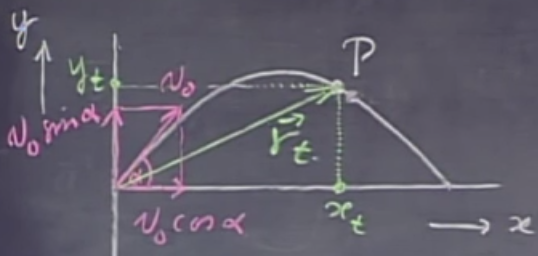
\includegraphics[scale=0.65]{\pIImages/2d-motion-decomposed}
\end{center}

The ball moves along the trajectory shown in white. It is launched (thrown) at an initial velocity $v_0$ (in magenta), which is a vector pointing at an angle $\alpha$ from the ground. Also in magenta, we have the initial velocities for the $x$ and $y$ directions, found via vector decomposition:

\begin{align}
v_{0x} &= v_0 \cos \alpha\\
v_{0y} &= v_0 \sin \alpha
\end{align}

Because there is no force acting on the ball in the $x$ direction, this is the velocity it will have in the $x$ direction until it hits the ground.\\
In green, the ball's position vector at a later point is shown, together with its $x$ and $y$ components, all three dependent on time $t$.

We can now apply the equations we found earlier, for one-dimensional motion under either constant acceleration or constant velocity. That is, these:

\begin{align}
x(t) &= x_0 + v_{0x} t + \frac{1}{2} a_x t^2\\
v_x(t) &= v_{0x} + a_x t
\end{align}

The same equations can of course be used for $y$ (and $z$) by simply replacing all $x$ terms with $y$ (or $z$).

With these equations in mind, we can now calculate the object's $x$ position at any moment in time as

\begin{equation}
x(t) = (v_0 \cos \alpha) t
\end{equation}

... since we are free to choose $x_0 = 0$, and there is no acceleration in the $x$ direction ($a_x = 0$).

This simple equation describes the $x$ position completely, from $t=0$ when it is launched, to whenever it hits the ground. To find out when that is, we need to calculate the $y$ position over time.

We use the same equations, with $y_0 = 0$	 (again, we are free to choose where we place our zero coordinate), and $a_y = -g$, that is, the gravitational acceleration of the Earth. $g$ is always positive, however, and in the diagram, we have chosen increasing $y$ to be upwards. Therefore we need to be careful and write $-g$ in this case, or we would be saying that gravity would accelerate the ball towards the sky!

We make the substitutions for the values ($y_0$ and $a_y$ as mentioned above, and the initial velocity in the $y$ direction is $v_0 \sin \alpha$ as we saw before)

\begin{align}
y(t) &= (v_0 \sin \alpha) t - \frac{1}{2} g t^2\\
v_y(t) &= v_0 \sin \alpha - g t
\end{align}

Note the minus sign for the acceleration.\\
The last three equations completely describe the ball's $x$ position, $y$ position, and $y$ velocity. The $x$ velocity is known to be constant.

Together, we can use the $x(t)$ and $y(t)$ equations to describe the trajectory:

\begin{align*}
x(t) &= (v_0 \cos \alpha) t\\
y(t) &= (v_0 \sin \alpha) t - \frac{1}{2} g t^2
\end{align*}

This is then demonstrated in lecture, by firing a golf ball straight up (as seen by the launcher), from a cart moving on a rail.\\
For an outside observer, such as us, the ball moves in a parabolic trajectory, and returns to the launcher a few seconds later, as they moved together at the constant $x$ velocity.\\
The successful demonstration concludes this lecture.
